\documentclass[a4paper,twoside]{article}
\usepackage[T1]{fontenc}
\usepackage[bahasa]{babel}
\usepackage{graphicx}
\usepackage{graphics}
\usepackage{float}
\usepackage[cm]{fullpage}
\pagestyle{myheadings}
\usepackage{etoolbox}
\usepackage{setspace} 
\usepackage{lipsum} 
\setlength{\headsep}{30pt}
\usepackage[inner=2cm,outer=2.5cm,top=2.5cm,bottom=2cm]{geometry} %margin
\graphicspath{ {./gambar/} }
% \pagestyle{empty}

\makeatletter
\renewcommand{\@maketitle} {\begin{center} {\LARGE \textbf{ \textsc{\@title}} \par} \bigskip {\large \textbf{\textsc{\@author}} }\end{center} }
\renewcommand{\thispagestyle}[1]{}
\markright{\textbf{\textsc{Laporan Perkembangan Pengerjaan Skripsi\textemdash Sem. Ganjil 2019/2020}}}

\onehalfspacing
 
\begin{document}

\title{\@judultopik}
\author{\nama \textendash \@npm} 

%ISILAH DATA BERIKUT INI:
\newcommand{\nama}{Hapsari Laksmi W}
\newcommand{\@npm}{2015730037}
\newcommand{\tanggal}{11/14/2019} %Tanggal pembuatan dokumen
\newcommand{\@judultopik}{Migrasi Zurb Foundation ke Bootstrap 4} % Judul/topik anda
\newcommand{\kodetopik}{PAN4791}
\newcommand{\jumpemb}{1} % Jumlah pembimbing, 1 atau 2
\newcommand{\pembA}{Pascal Alfadian .N}
\newcommand{\pembB}{-}
\newcommand{\semesterPertama}{47 - Ganjil 19/20} % semester pertama kali topik diambil, angka 1 dimulai dari sem Ganjil 96/97
\newcommand{\lamaSkripsi}{1} % Jumlah semester untuk mengerjakan skripsi s.d. dokumen ini dibuat
\newcommand{\kulPertama}{Skripsi 1} % Kuliah dimana topik ini diambil pertama kali
\newcommand{\tipePR}{B} % tipe progress report :
% A : dokumen pendukung untuk pengambilan ke-2 di Skripsi 1
% B : dokumen untuk reviewer pada presentasi dan review Skripsi 1
% C : dokumen pendukung untuk pengambilan ke-2 di Skripsi 2

% Dokumen hasil template ini harus dicetak bolak-balik !!!!

\maketitle

\pagenumbering{arabic}

\section{Data Skripsi} %TIDAK PERLU MENGUBAH BAGIAN INI !!!
Pembimbing utama/tunggal: {\bf \pembA}\\
Pembimbing pendamping: {\bf \pembB}\\
Kode Topik : {\bf \kodetopik}\\
Topik ini sudah dikerjakan selama : {\bf \lamaSkripsi} semester\\
Pengambilan pertama kali topik ini pada : Semester {\bf \semesterPertama} \\
Pengambilan pertama kali topik ini di kuliah : {\bf \kulPertama} \\
Tipe Laporan : {\bf \tipePR} -
\ifdefstring{\tipePR}{A}{
			Dokumen pendukung untuk {\BF pengambilan ke-2 di Skripsi 1} }
		{
		\ifdefstring{\tipePR}{B} {
				Dokumen untuk reviewer pada presentasi dan {\bf review Skripsi 1}}
			{	Dokumen pendukung untuk {\bf pengambilan ke-2 di Skripsi 2}}
		}
		
\section{Latar Belakang}
BlueTape merupakan aplikasi berbasis \textit{web} yang berfungsi mengolah beberapa kebutuhan administrasi fakultas secara \textit{paperless} yang digunakan dalam lingkungan FTIS UNPAR.  Aplikasi ini mempunyai fitur untuk manajemen transkrip nilai, perubahan kuliah dan jadwal dosen. \textit{Framework} yang digunakan dalam aplikasi BlueTape ada dua yaitu \textit{Codeigniter} dan \textit{Zurb Foundation}.  

\begin{figure}[h]
	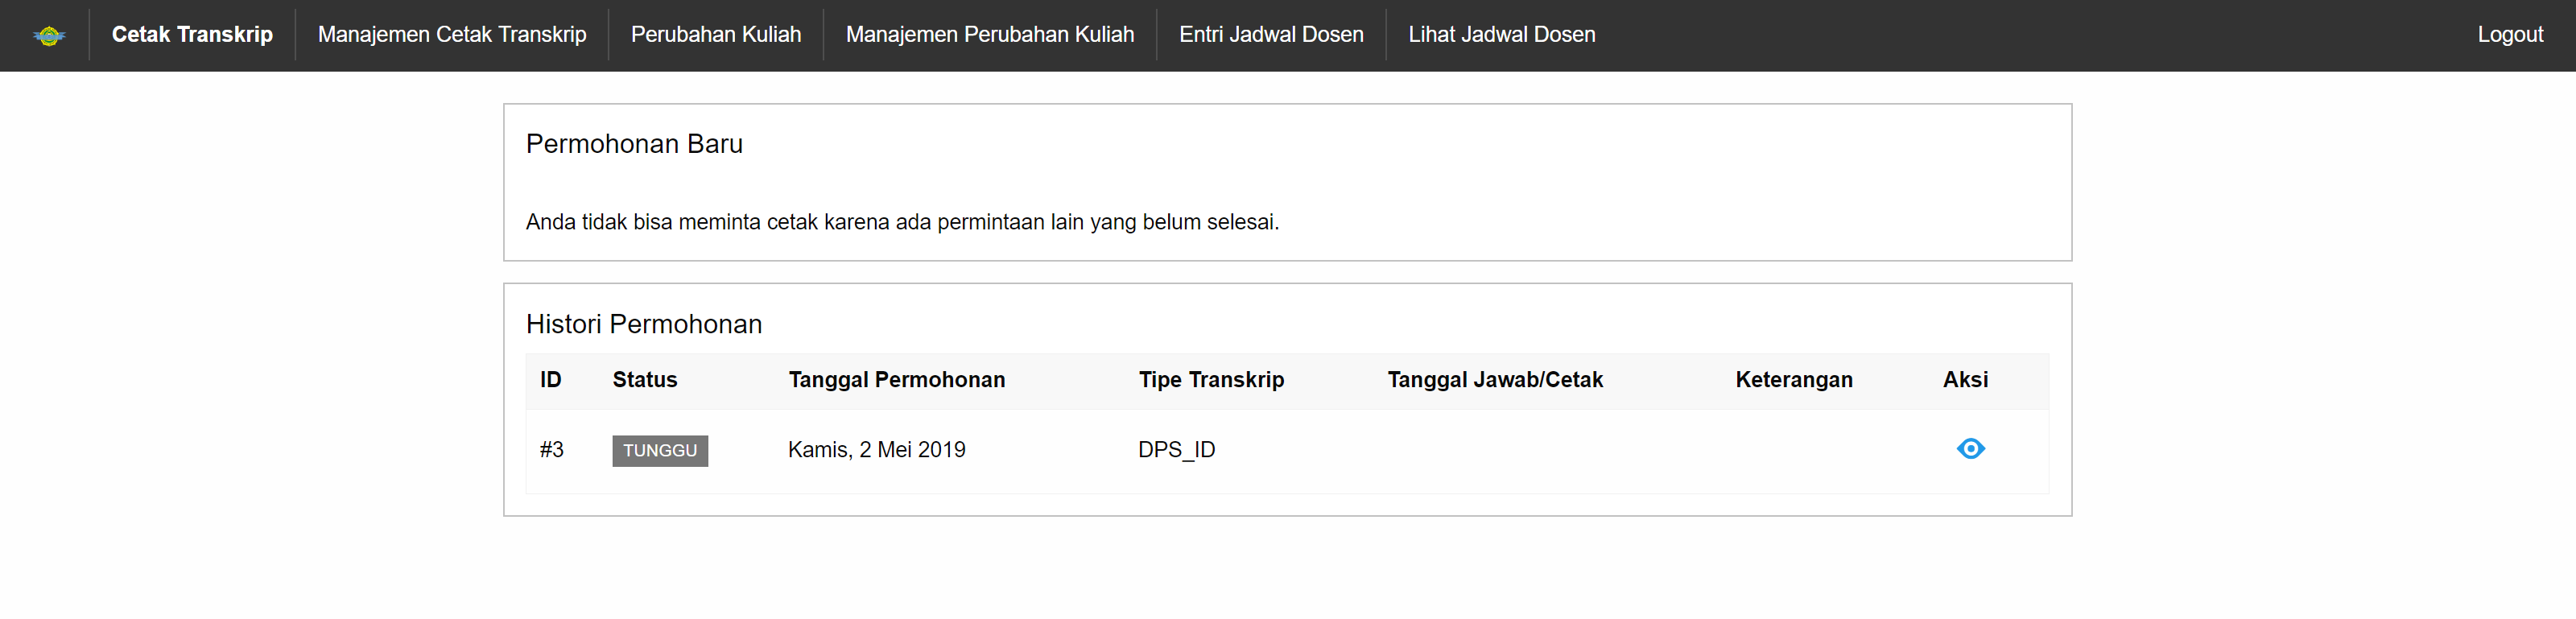
\includegraphics [scale=0.5] {Tampilan-Cetak-Transkrip.PNG}
	\caption{Tampilan Cetak Transkrip}
\end{figure}

\begin{figure}[h]
	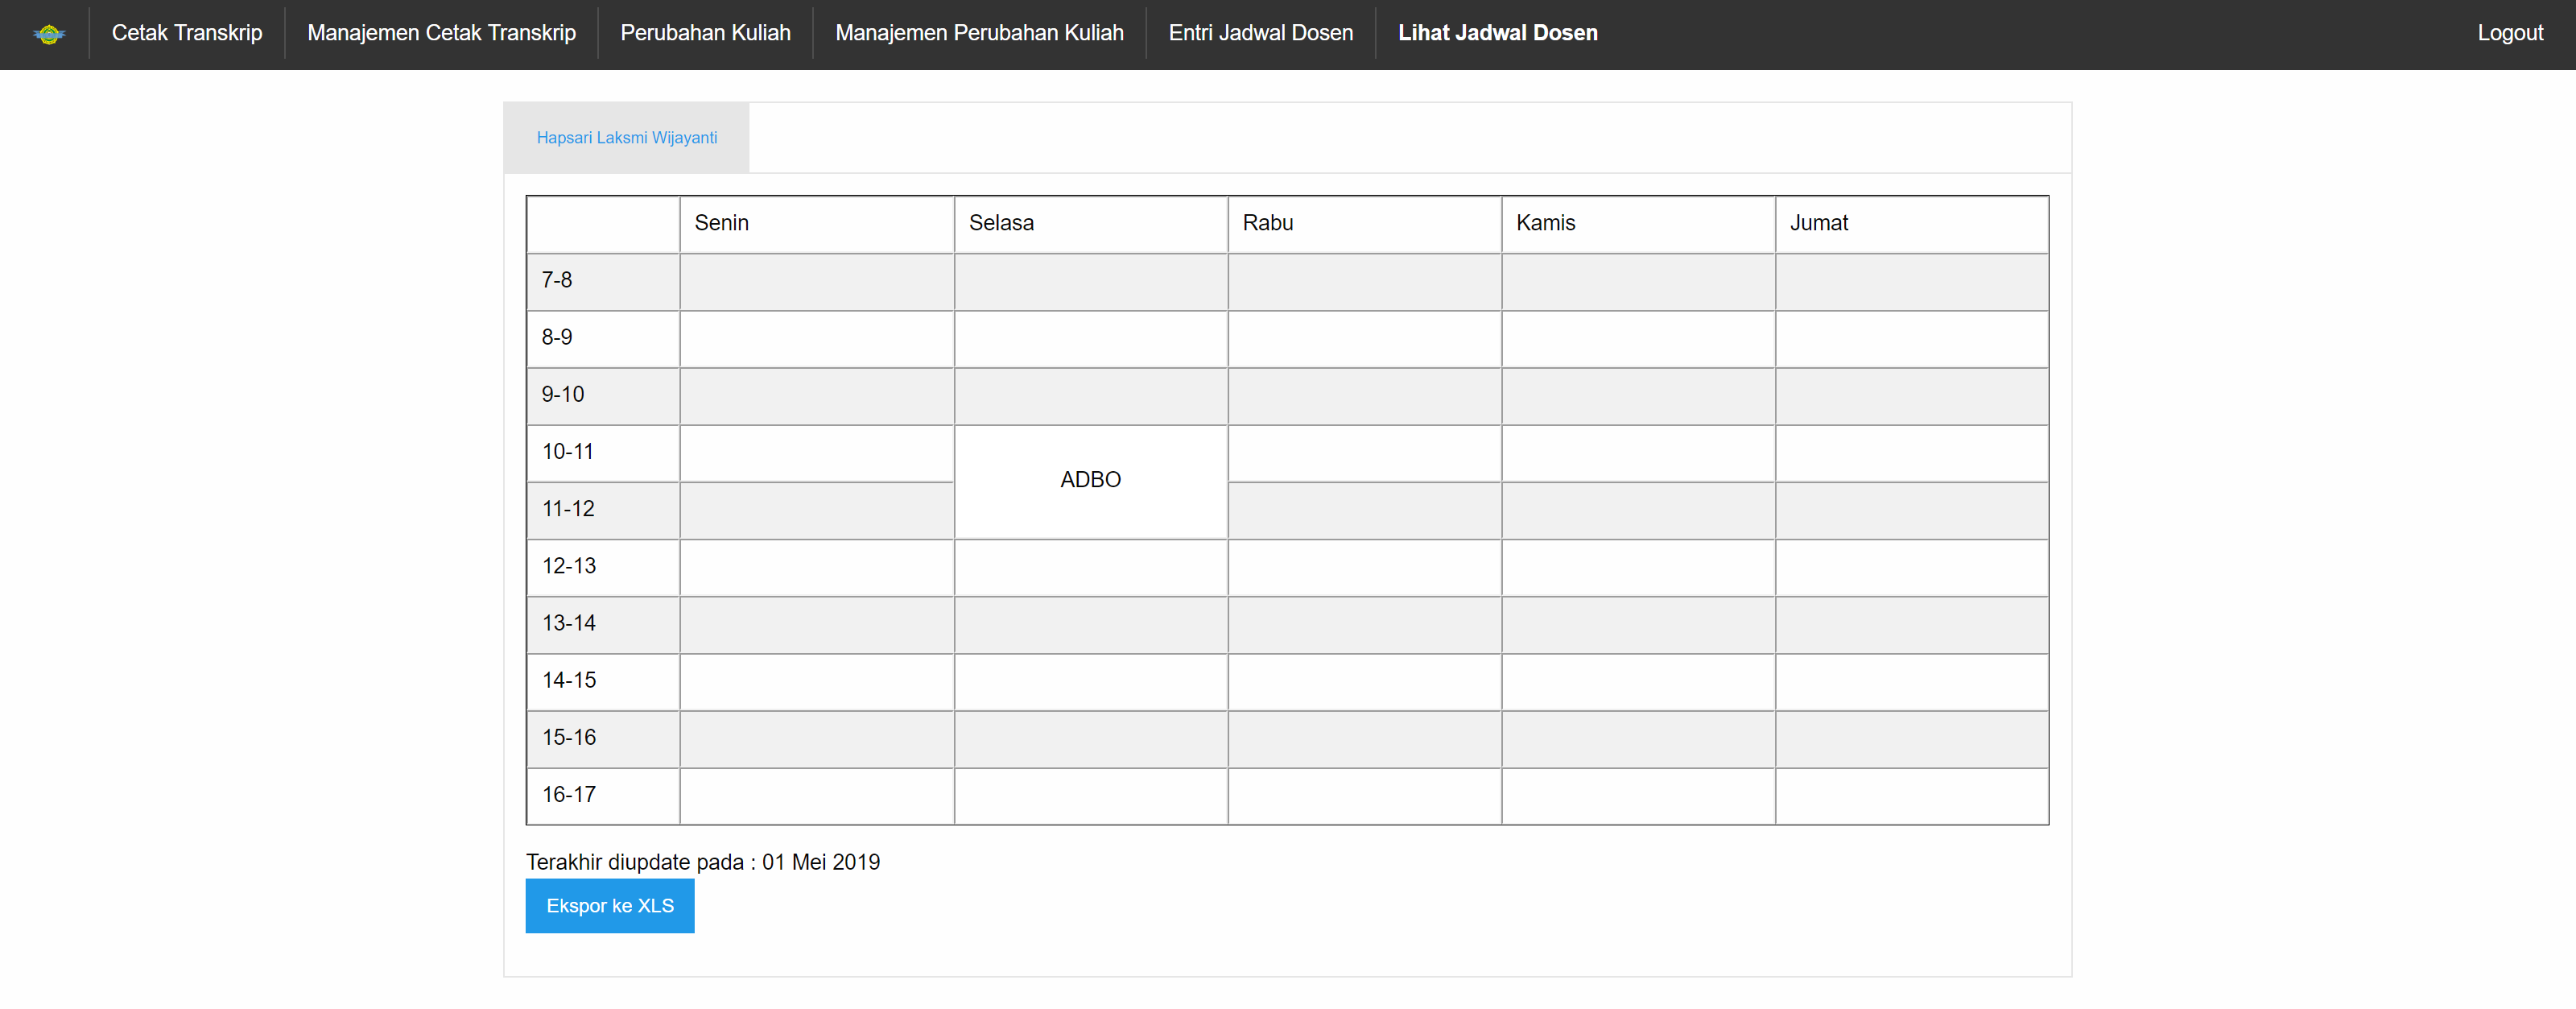
\includegraphics [scale=0.5] {Tampilan-Lihat-Jadwal-Dosen.PNG}
	\caption{Tampilan Lihat Jadwal Dosen}
\end{figure}

\begin{figure}[h]
	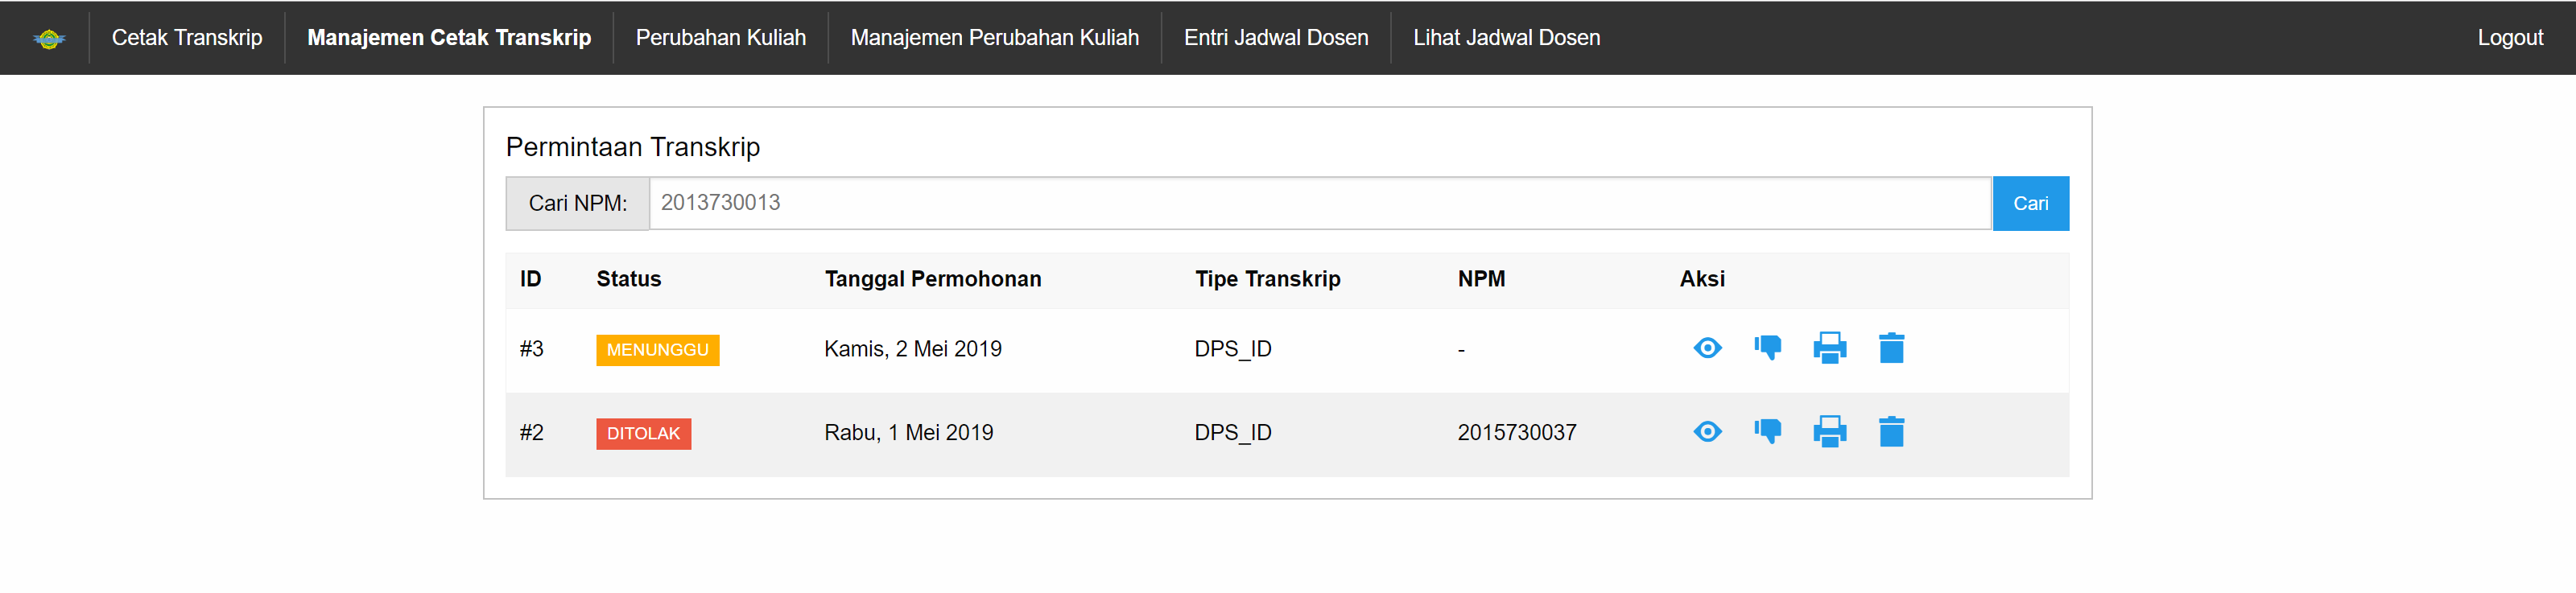
\includegraphics [scale=0.5] {Tampilan-Manajemen-Cetak-Transkrip.PNG}
	\caption{Tampilan-Manajemen-Cetak-Transkrip}
\end{figure}

\begin{figure}[h]
	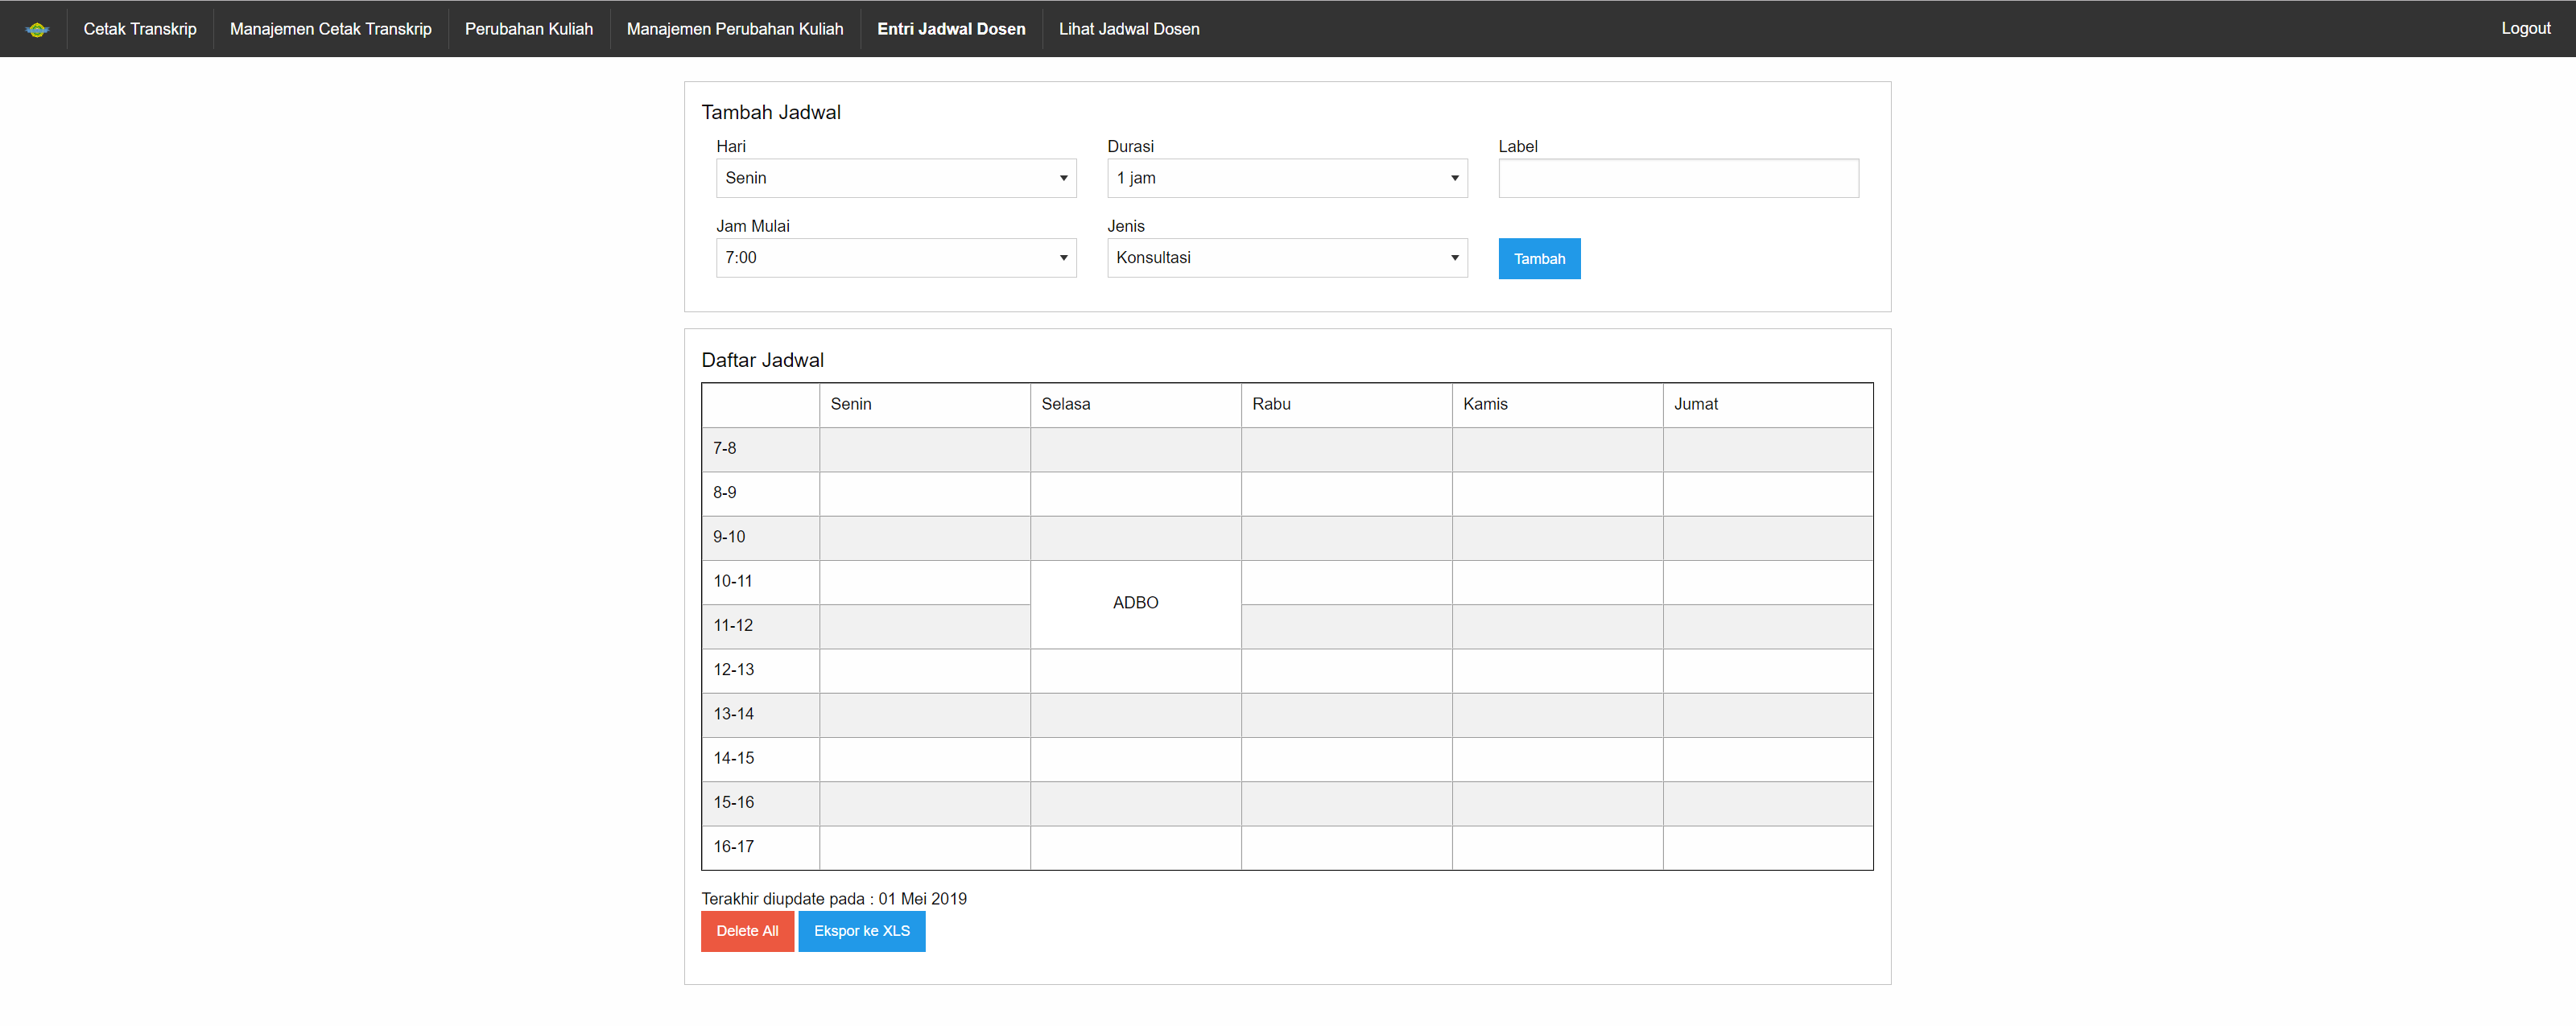
\includegraphics [scale=0.5] {Tampilan-Entri-Jadwal-Dosen.PNG}
	\caption{Tampilan Entri Jadwal Dosen}
\end{figure}

\begin{figure}[ht!]
	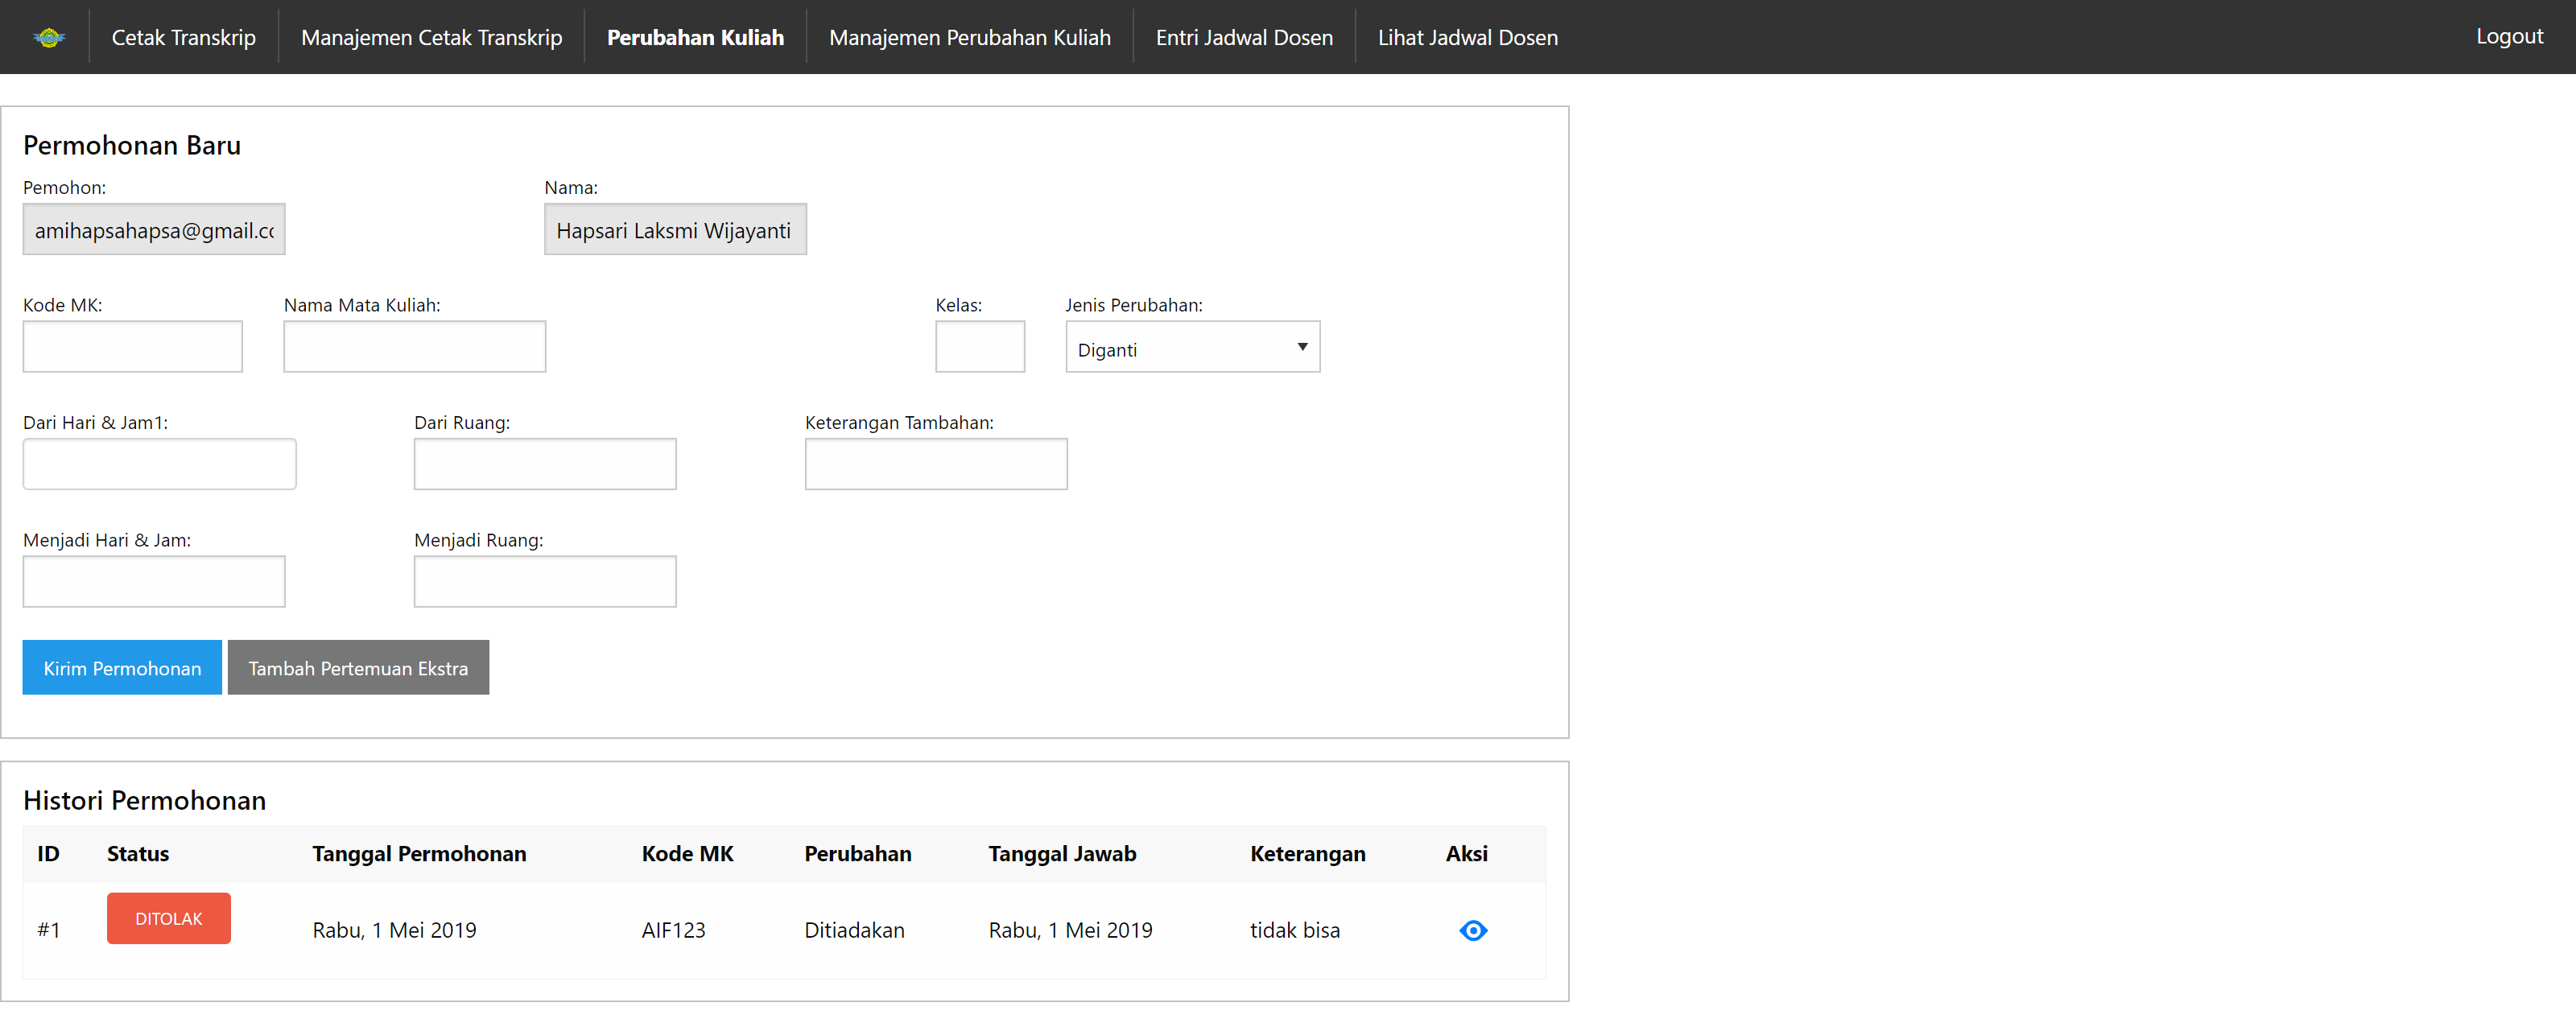
\includegraphics [scale=0.5] {Tampilan-Perubahan-Kuliah.PNG}
	\caption{Tampilan Perubahan Kuliah}
\end{figure}

\begin{figure}[ht!]
	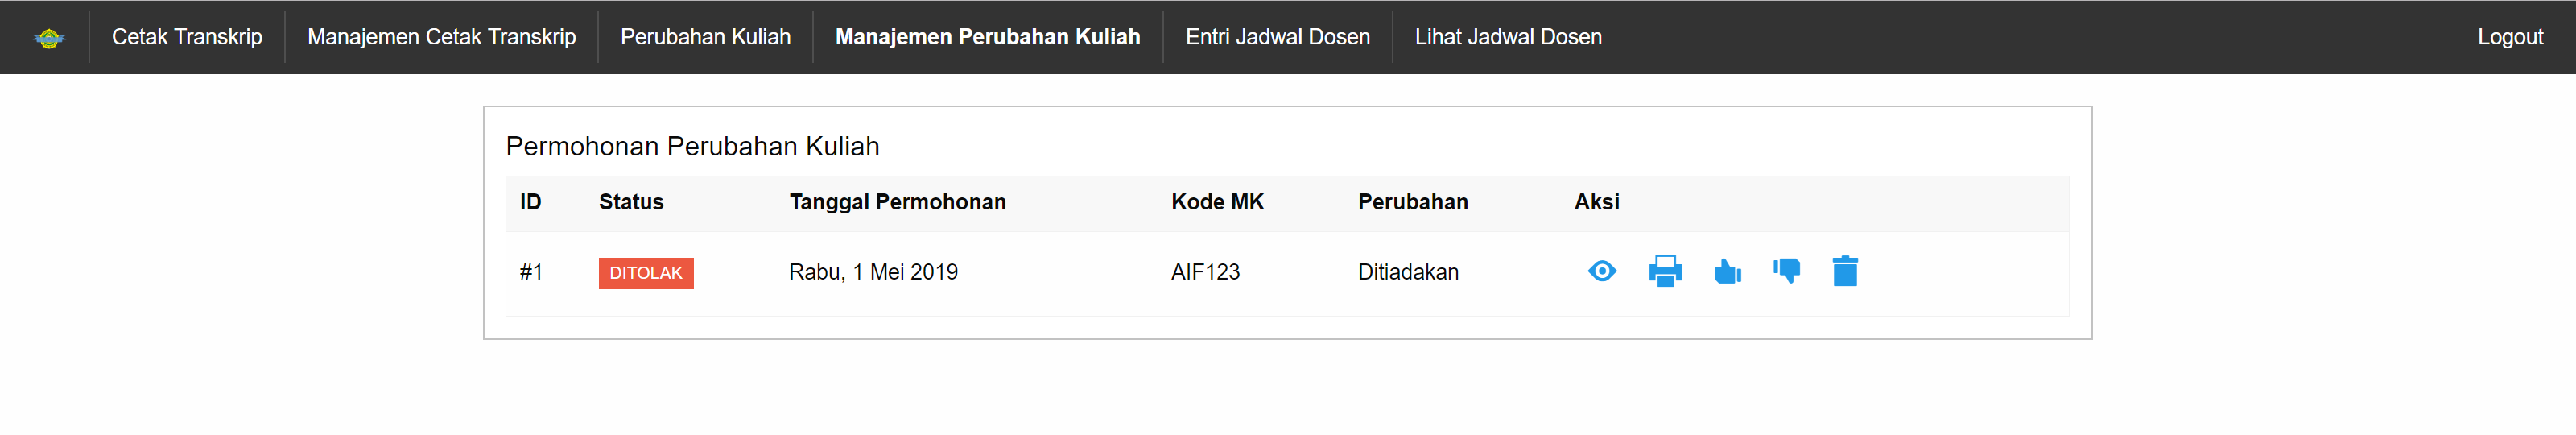
\includegraphics [scale=0.5] {Tampilan-Manajemen-Perubahan-Kuliah.PNG}
	\caption{Tampilan Manajemen Perubahan Kuliah}
\end{figure}




Meskipun \textit{open-source}, saat ini \textit{Zurb Foundation} tidak sepopuler \textit{framework} \textit{Bootstrap}. 
\textit{Bootstrap} adalah \textit{ Javascript framework} yang didesain untuk membantu membangun komponen \textit{user interface} yang terdiri dari \textit{CSS, JavaScript/jQuery}, dan \textit{glyphicons}. Pembangunan \textit{website} yang lebih cepat dan besarnya komunitas yang ada berdampak pada banyaknya pengembang \textit{web} yang memanfaatkan \textit{framework Bootstrap}. Sehingga jumlah proyek yang dihasilkan oleh\textit{ framework Bootstrap} lebih banyak dibanding \textit{Zurb Foundation}. 

\section{Tujuan}
Tujuan yang ingin dicapai dalam penelitian ini :
\begin{enumerate}
	\item Membuat template cetak transkrip nilai, template manajemen cetak transkrip, template perubahan kuliah, module manajemen perubahan kuliah, modul entri jadwal dosen dan module lihat jadwal dosen dengan framework Bootstrap 4 yang responsive untuk berbagai platform.
	\item Mengimplentasikan plugin yang tersedia dalam library Bootstrap 4.	
\end{enumerate}

\section{Rumusan Masalah}
\begin{enumerate}
	\item Bagaimana membuat template manajemen cetak transkrip, manajemen perubahan kuliah dan manajemen jadwal dosen.
	\item Bagaimana mengimplentasikan plugin yang tersedia di dalam Bootstrap 4.	
\end{enumerate}

\section{Detail Perkembangan Pengerjaan Skripsi}
Detail bagian pekerjaan skripsi sesuai dengan rencan kerja/laporan perkembangan terkahir :
	\begin{enumerate}
		\item \textbf{Mempelajari framework PHP Codeigniter.}\\
		{\bf Status :} Ada sejak rencana kerja skripsi.\\
		{\bf Hasil :} Mempelajari konsep codeigniter dan mencoba langsung didalam projek BlueTape
		
		\item \textbf{Mempelajari framework front-end Bootstrap 4 beserta plugin-plugin yang tersedia.}\\
		{\bf Status :} Ada sejak rencana kerja skripsi.\\
		{\bf Hasil :} Sudah dicoba pada sebagian besar projek BlurTape.

		\item \textbf{Membuat rancangan tampilan website dan template.}\\
		{\bf Status :} Ada sejak rencana kerja skripsi.\\
		{\bf Hasil :} Rancangan sebagian sudah dijelaskan

		\item \textbf{Mengimplementasikan keseluruhan rancangan tampilan dan template.}\\
		{\bf Status :} Ada sejak rencana kerja skripsi.\\
		{\bf Hasil :} Sebagian besar tampilan sudah diimplementasi

		\item \textbf{Menulis dokumen skripsi.}\\
		{\bf Status :} Ada sejak rencana kerja skripsi.\\
		{\bf Hasil :} Mengerjakan bab 1, bab 2 dan bab 3
	\end{enumerate}

\section{Pencapaian Rencana Kerja}
Langkah-langkah kerja yang berhasil diselesaikan dalam Skripsi 1 ini adalah sebagai berikut:
\begin{enumerate}
	\item Mempelajari framework PHP Codeigniter.
	\item Mempelajari framework front-end Bootstrap 4 beserta plugin-plugin yang tersedia.
	\item Menulis dokumen skripsi.
\end{enumerate}
\begin{center}
	\begin{tabular}{|c|c|c|c|c|} 
		\hline
		1* & 2*(\%) & 3*(\%) & 4*(\%) & 5*(\%) \\ [0.5ex] 
		\hline\hline
		1 & 10 & 5 & 5 & memahami konsep MVC pada codeigniter pada projek BlueTape\\ 
		\hline
		2 & 20 & 5 & 15 & plugin baru diterapkan, belum menggunakan fitur yang sesuai \\
		\hline
		3 & 10 & 5 & 5 &  rancangan dijelaskan pada bab analisis\\
		\hline
		4 & 30 & 20 & 10 & sebagian besar antarmuka diterapkan\\
		\hline
		5 & 30 & 10 & 20 & sebagian besar bab 1, bab 2 dan sebagian kecil bab 3\\ [1ex] 
		\hline
		Total & 100 & 60 & 40 & \\ [1ex] 
		\hline
	\end{tabular}
\end{center}
Keterangan (*)
\begin{itemize}
	\item [$ $] 1 : Bagian pengerjaan Skripsi (nomor disesuaikan dengan detail pengerjaan di bagian 5)
	\item [$ $] 2 : Persentase total
	\item [$ $] 3 : Persentase yang akan diselesaikan di Skripsi 1
	\item [$ $] 4 : Persentase yang akan diselesaikan di Skripsi 2
	\item [$ $] 5 : Penjelasan singkat apa yang dilakukan di S1 (Skripsi 1) atau S2 (skripsi 2)	
\end{itemize}

\section{Kendala yang Dihadapi}
%TULISKAN BAGIAN INI JIKA DOKUMEN ANDA TIPE A ATAU C
Kendala - kendala yang dihadapi selama mengerjakan skripsi :
\begin{itemize}
	\item Sulit mengubah lebar cell dalam tabel.
\end{itemize}

\vspace{1cm}
\centering Bandung, \tanggal\\
\vspace{2cm} \nama \\ 
\vspace{1cm}

Menyetujui, \\
\ifdefstring{\jumpemb}{2}{
\vspace{1.5cm}
\begin{centering} Menyetujui,\\ \end{centering} \vspace{0.75cm}
\begin{minipage}[b]{0.45\linewidth}
% \centering Bandung, \makebox[0.5cm]{\hrulefill}/\makebox[0.5cm]{\hrulefill}/2013 \\
\vspace{2cm} Nama: \pembA \\ Pembimbing Utama
\end{minipage} \hspace{0.5cm}
\begin{minipage}[b]{0.45\linewidth}
% \centering Bandung, \makebox[0.5cm]{\hrulefill}/\makebox[0.5cm]{\hrulefill}/2013\\
\vspace{2cm} Nama: \pembB \\ Pembimbing Pendamping
\end{minipage}
\vspace{0.5cm}
}{
% \centering Bandung, \makebox[0.5cm]{\hrulefill}/\makebox[0.5cm]{\hrulefill}/2013\\
\vspace{2cm} Nama: \pembA \\ Pembimbing Tunggal
}
\end{document}

